% !TeX spellcheck = ru_RU
% !TEX root = vkr.tex

\section{Эксперимент}

В данном разделе представлены результаты экспериментального исследования алгоритмов для обработки изображений на GPU и CPU. Основные задачи исследования --- оценить производительность различных подходов к обработке изображений в условиях, близких к реальным, сравнить полученные показатели и ответить на  на вопрос, приведённый ниже.

\begin{itemize}
    \item[\textbf{RQ1:}] При каких размерах изображения фильтр Gauss выгоднее применять на CPU, а при каких на GPU?
\end{itemize}

\subsection{Условия эксперимента}

Эксперименты проводились на рабочей станции со следующими характеристиками.
\begin{itemize}
    \item Центральный процессор: AMD Ryzen 5 5600X 
    \item Видеокарта: NVIDIA GeForce RTX 3060
    \item Операционная система: Windows 11 Pro 22H2
\end{itemize}

\subsection{Набор данных}

Для замеров производительности использовались 4 вариации одного и того же цветного квадратного изображения формата .jpg различных размеров с сайта Sample Vi\-de\-os\footnote{Сайт с изображениями: \url{https://sample-videos.com/}.}. В табл. \ref{tbl:images} представлена информация об используемых данных: порядковый номер изображения, название и размер в пикселях.

\begin{table}
\centering
\caption{Параметры изображений}
\label{tbl:images}
\rowcolors{2}{black!2}{black!10}
\scalebox{0.7}{
\begin{tabular}{|c|p{7cm}|c|}
\hline
Номер & Название & Размер \\
\hline
\hline
1 & SampleJPGImage_50kbmb & 300 x 300 \\
2 & SampleJPGImage_100kbmb & 689 x 689 \\
3 & SampleJPGImage_200kbmb & 1036 x 1036 \\
4 & SampleJPGImage_500kbmb & 1792 x 1792 \\
\hline
\end{tabular}
}
\end{table}

\subsection{Метрики}

В исследовании для замеров производительности была использована библиотека Bench\-mark\-Dot\-Net~v0.13.4\footnote{Библиотека BenchmarkDotNet для замеров производительности: \url{https://benchmarkdotnet.org/}.}. В качестве метрик производительности выступает время, требуемое для выполнения операции. Предварительно совершался не учитывающийся в замерах прогревочный запуск, содержащий от 6 до 50 итераций (точное количество рассчитывается с помощью эвристики). Показатели времени усреднены по количеству целевых итераций; минимальное количество итераций 15, максимальное --- 100 (точное количество рассчитывается с помощью эвристики). Стандартное отклонение (StdDev) составляет не более 10\% от среднего значения (mean) для каждого отдельного эксперимента. Гистограмма приведена на рис. \ref{fig:hist}.

\begin{figure}
    \centering
    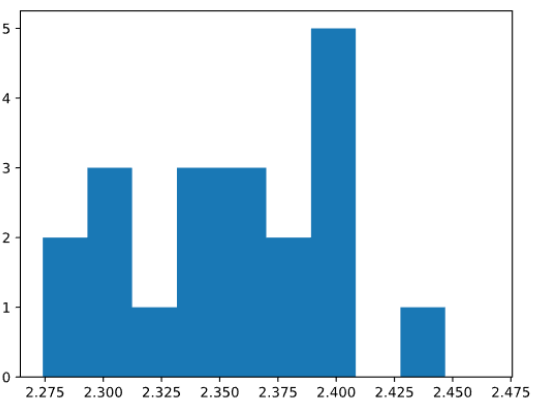
\includegraphics[width=0.6\textwidth]{hist.png}
    \caption{Гистограмма со значениями: $pvalue \approx 0.61$, $pvalue \approx 0.67$}
    \label{fig:hist}
\end{figure}

\subsection{Результаты}

Столбчатая диаграмма, реализованные с помощью Mat\-plot\-lib, на рис. \ref{fig:bar} иллюстрирует результаты экспериментального исследования. На оси абсцисс отмечены размеры исследуемых изображений, на оси ординат представлены двойные столбцы --- оранжевым отмечен результат работы CPU, в каждом случае принимаемый за единицу, синим --- ускорение, равное отношению значения полученного при обработке исходного изображения на GPU к CPU. Данный вид диаграммы позволяет компактно изобразить все полученные данные.

\textit{RQ1: При каких размерах изображения фильтр Gauss выгоднее применять на CPU, а при каких на GPU?}

Во всех случаях, оказалось выгоднее использовать GPU для обработки изображения с помощью фильтра Gauss, отрыв между ними настолько большой, что столбец CPU на диаграмме практически не виден. Наибольшее ускорение (на изображении размера 1792 x 1792) достигло значения в 475 раз, минимальное --- в 48 раз (на изображении размера 300 x 300).

\begin{landscape}
\begin{figure}
    \thispagestyle{empty} 
    \centering
    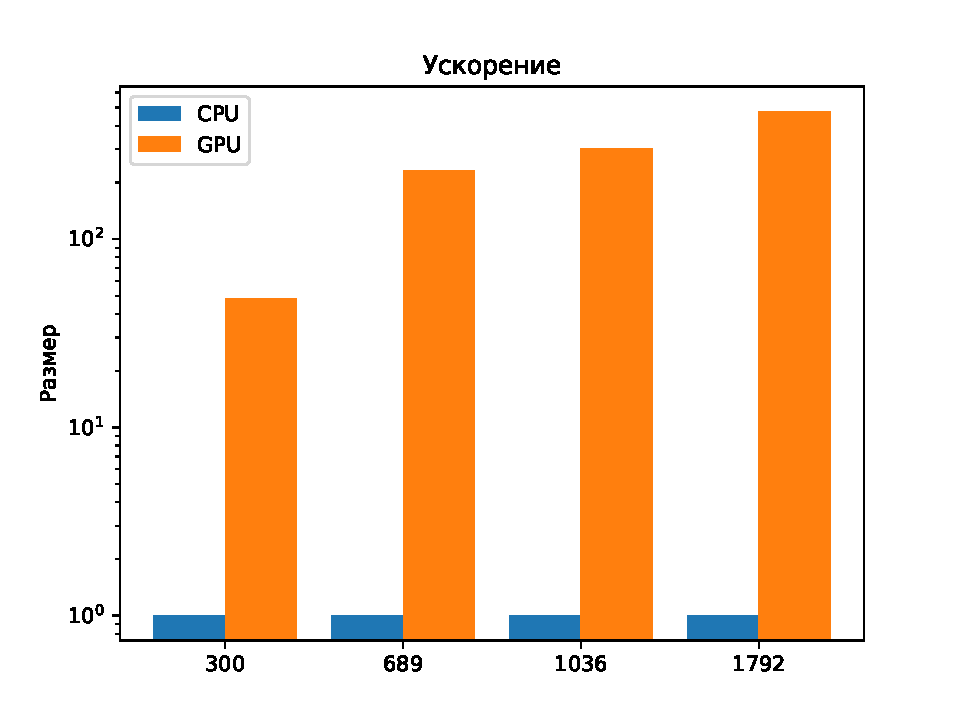
\includegraphics[height=0.8\textwidth]{figures/bar.pdf}
    \caption{Результаты применения фильтра на GPU и CPU\\}
    \label{fig:bar}
\end{figure}
\end{landscape}